% The circle $ included into the ambient plane $\mathbb{R}^2$.
% Source: book/tex/riemann-surface/affine-projective.tex (§ Varieties as intrinsic objects).
\documentclass[border=2mm]{standalone}
\usepackage{tikz}
\usepackage{amssymb}
\usetikzlibrary{arrows.meta}
\begin{document}
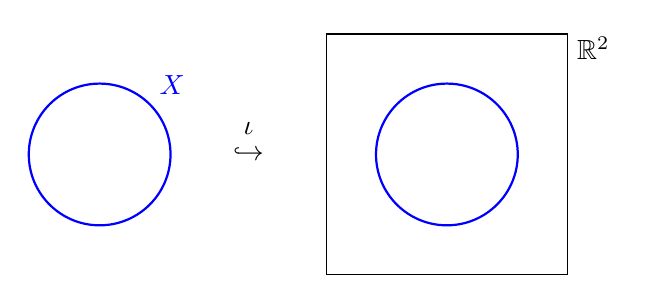
\begin{tikzpicture}[>=Latex,scale=0.9]
\draw[blue,thick](0,0)circle(1);\node[blue,above right]at(45:1){$X$};
\node at(2.1,0){$\hookrightarrow$};\node[above]at(2.1,0.15){$\iota$};
\draw(3.2,-1.7)rectangle(6.6,1.7);\node[right]at(6.6,1.5){$\mathbb{R}^2$};\draw[blue,thick](4.9,0)circle(1);
\end{tikzpicture}
\end{document}
